% Unofficial Georgia Tech Psychology Poster Template
% based on
% https://github.com/k4rtik/uchicago-poster
% a fork of https://github.com/anishathalye/gemini

\documentclass[final]{beamer}

% ====================
% Packages
% ====================

\usepackage[T1]{fontenc}
\usepackage{lmodern}
\usepackage[size=custom,width=120,height=95,scale=1.0]{beamerposter}
\usetheme{gemini}
\usecolortheme{gatech}
\usepackage{graphicx}
\usepackage{booktabs}
\usepackage{doi}
\usepackage{natbib}
\usepackage[patch=none]{microtype}
\usepackage{tikz}
\usepackage{qrcode}
\usepackage{pgfplots}
\usepackage{subfig}
\pgfplotsset{compat=1.18}
\usepackage{anyfontsize}

\pdfstringdefDisableCommands{%
\def\translate#1{#1}%
}

% ====================
% Lengths
% ====================

% If you have N columns, choose \sepwidth and \colwidth such that
% (N+1)*\sepwidth + N*\colwidth = \paperwidth
\newlength{\sepwidth}
\newlength{\colwidth}
\setlength{\sepwidth}{0.025\paperwidth}
\setlength{\colwidth}{0.3\paperwidth}

\newcommand{\separatorcolumn}{\begin{column}{\sepwidth}\end{column}}

% ====================
% Title
% ====================

\title{Weierstrass-Enneper Parametrization of Minimal Surfaces (MATH 419)}

\author{\LARGE\textbf{Jimmy Sitompul}}


% ====================
% Footer (optional)
% ====================

\footercontent{
  \Large \textbf{Department of Mathematics} \hfill \Large \textbf{Colorado State University}
  \hfill
  \href{mailto:jimmy.sitompul@colostate.edu}{jimmy.sitompul@colostate.edu}}
% (can be left out to remove footer)

% ====================
% Logo (optional)
% change logos in header by replacing the png files
% ====================


% ====================
% Body
% ====================

\begin{document}
\addtobeamertemplate{headline}{}
{
    \begin{tikzpicture}[remember picture, overlay]
      \node [anchor=north west, inner sep=3cm] at ([xshift=0.0cm,yshift=2.5cm]current page.north west)
      {
\includegraphics[height=6.0cm]{Math-NS-CSU-1-H357.png}};
      \node [anchor=north east, inner sep=3cm] at ([xshift=0.0cm,yshift=2.5cm]current page.north east)
      {
\includegraphics[height=6.0cm]{Math-NS-CSU-1-H357.png}};
    \end{tikzpicture}
}

\begin{frame}[t]
\begin{columns}[t]
\separatorcolumn

\begin{column}{\colwidth}

  \begin{alertblock}{What Are Minimal Surfaces?}
      Minimal surfaces are geometric objects with intriguing features that can be explored using computers. Minimal surfaces minimize surface area locally, and these surfaces arises as these surfaces subject to some boundary constraint. Formally, a minimal surface $M$ with mean curvature $H=0$ at all points $p \in M$. 
  \end{alertblock}
\vspace{\baselineskip}
  \begin{block}{Examples of Minimal Surfaces}
   The following figures are examples of minimal surfaces, both embedded and unembedded minimal surfaces.
   \vspace{\baselineskip}
   \begin{figure}
       \centering
       \subfloat[\centering Plane]{{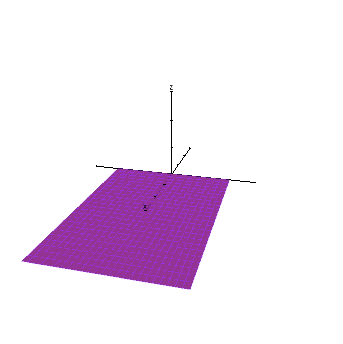
\includegraphics[scale=2.5]{graphs/plane.png} }}
       \subfloat[\centering Helicoid]{{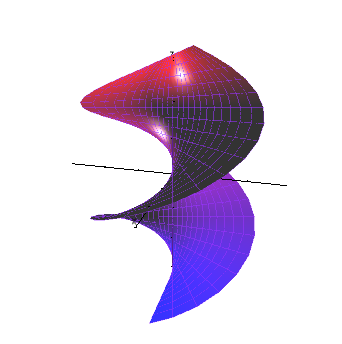
\includegraphics[scale=2.5]{graphs/helicoid.png} }}
       \subfloat[\centering Catenoid]{{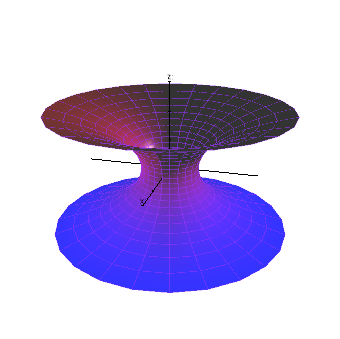
\includegraphics[scale=2.5]{graphs/catenoid.png} }}
       \caption{The Graphs of Embedded Minimal Surfaces}
   \end{figure}
   \begin{figure}
       \centering
       \subfloat[\centering Enneper Surface]{{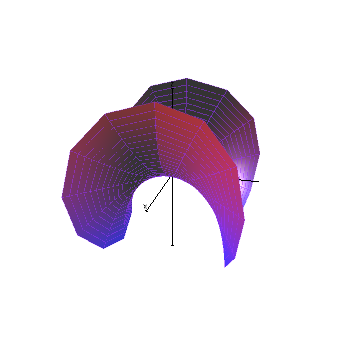
\includegraphics[scale=2.5]{graphs/Enneper.png} }}
       \subfloat[\centering Henneberg Surface]{{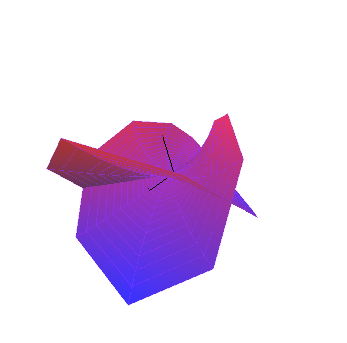
\includegraphics[scale=2.5]{graphs/Henneberg.png }}}
       \subfloat[\centering Catalan Surface]{{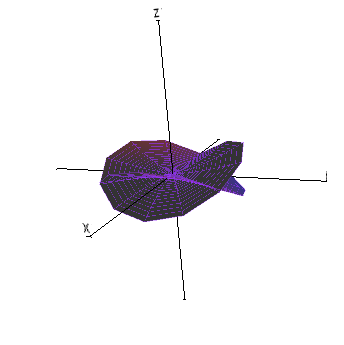
\includegraphics[scale=2.5]{graphs/Catalan.png} }}
       \caption{The Graphs of Unembedded Minimal Surfaces}
   \end{figure}
  \end{block}
  \vspace{\baselineskip}
  \vspace{\baselineskip}
  \begin{alertblock}{Holomorphic Functions And Minimal Surfaces Relationship}

    Here, the concept of complex analysis, namely holomorphic functions, is helpful for learning more about minimal surfaces, because holomorphic functions are the necessary and sufficient condition for a surface to be minimal. The following theorem that uses the properties of an isothermal parametrization will lead to the desired condition.\\
    \vspace{\baselineskip}
    \textbf{Theorem 1.} A parametrization $\textbf{x}(u,v)$ is \emph{isothermal} if $E=\textbf{x}_u \cdot \textbf{x}_u = \textbf{x}_v \cdot \textbf{x}_v = G$ and $F= \textbf{x}_u \cdot \textbf{x}_v=0$.\\
    \vspace{\baselineskip}
    \textbf{Theorem 2.} If the parametrization $\textbf{x}$ is isothermal, then
    \begin{align*}
        \textbf{x}_{uu} +\textbf{x}_{vv}=2EH\textbf{n}
    \end{align*}
    where E is a coefficient of the first fundamental form and H is the mean curvature.\\
    \vspace{\baselineskip}
    Since $H=0$ for a minimal surface, the theorem above tells us that $\textbf{x}_{uu} +\textbf{x}_{vv}=0$. But what does this equation represent? It represents the Laplace equation that is satisfied by a harmonic function $u$ and therefore we have the following theorem.\\
    \vspace{\baselineskip}
    \textbf{Theorem 3.} A surface $M$ with an isothermal parametrization $\textbf{x}(u,v)=(x_1(u,v),x_2(u,v),x_3(u,v))$ is minimal if and only if $x_1,x_2,x_3$ are harmonic.\\
    \vspace{\baselineskip}
    In addition to the theorem above, let $\phi=(\varphi_1,\varphi_2,\varphi_3)$, where $\varphi_k=\frac{\partial x_k}{\partial z}$, then $M$ is minimal if and only if each $\varphi_k$ is holomorphic.\\
    These theorems above are the foundations to establish the Weierstrass representation for minimal surface, therefore holomorphic and harmonic functions are the necessary and sufficient conditions for a surface to be minimal.
    \vspace{\baselineskip}
  \end{alertblock}

\end{column}

\separatorcolumn

\begin{column}{\colwidth}

\begin{alertblock}{Weierstrass-Enneper Parametrization Theorem}

    Suppose $p$ is a holomorphic function and $q$ is a meromorphic function in some domain $\Omega \subset \mathbb{C}$, with the property that at each point where $q$ has a pole of order $m$, $p$ has a zero of order at least $2m$, and $a \in \Omega$ is a constant. Every regular minimal surface has a local isothermal parametric representation of the form
    \begin{flalign*}
        \textbf{x} &= (x_1(z),x_2(z),x_3(z))\\
        &= \Big{(} \text{Re} \Big {\{} \int_{a}^{z} p(1+q^2)dz \Big {\}}, \text{Re} \Big {\{} \int_{a}^{z} -ip(1-q^2)dz \Big {\}}, \text{Re} \Big {\{} \int_{a}^{z} -2ipqdz \Big {\}} \Big{)}
    \end{flalign*}
    where $p$, $pq^2$, and $pq$ are holomorphic.
  \end{alertblock}
\vspace{\baselineskip}
  \begin{block}{Weierstrass-Enneper Parametrization: Unembedded Minimal Surfaces}
    \heading{Enneper Surface Representation}
    Suppose $p(z)=1$ and $q(z)=iz$, we will show that this generates the Enneper surface. We get, 
    \begin{flalign*}
        \textbf{x}&= \Big{(} \text{Re} \Big {\{} \int_{0}^{z} (1-z^2)dz \Big {\}}, \text{Re} \Big {\{} \int_{0}^{z} -i(1+z^2)dz \Big {\}}, \text{Re} \Big {\{} \int_{0}^{z} 2zdz \Big {\}} \Big{)}\\
        &= \Big{(} \text{Re} \Big {\{} z- \frac{1}{3}z^3 \Big {\}}, \text{Re} \Big {\{} -i \Big{(} z+ \frac{1}{3}z^3 \Big{)} \Big {\}}, \text{Re} \Big {\{} z^2 \Big{\}} \Big{)}
    \end{flalign*}
    \vspace{\baselineskip}
    Letting $z=u+iv$, this yields
    \begin{align*}
        \textbf{x}(u,v) = \Big{(} u-\frac{1}{3}u^3 +uv^2, v -\frac{1}{3}v^3 +u^2 v, u^2-v^2 \Big{)}
    \end{align*}
    \vspace{\baselineskip}
    which gives the Enneper surface.\\
    The graph of this minimal surface can be visualized by using the applet \emph{MinSurfTool} by putting $p(z)=1$ and $q(z)=i*z$ in the appropriate boxes in the following figure.
    \vspace{\baselineskip}
    \begin{figure}
        \centering
        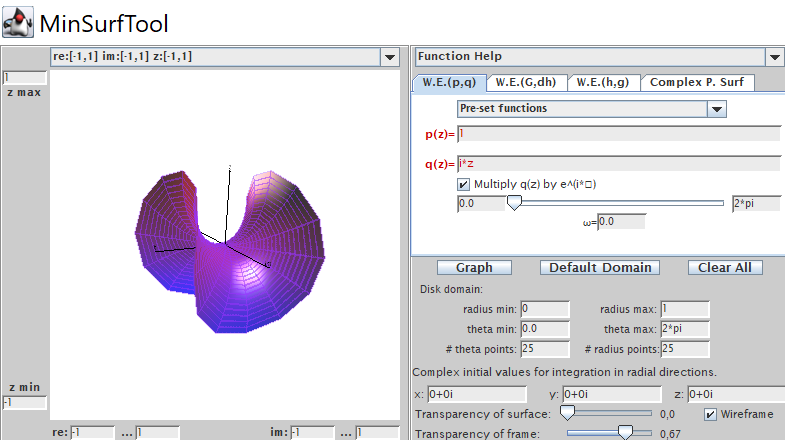
\includegraphics[scale=3]{graphs/EnneperGraph.png}
        \caption{Enneper surface using $p(z)=1$ and $q(z)=iz$.}
        \label{fig:my_label}
    \end{figure}
  \end{block}
  \vspace{\baselineskip}

  \begin{alertblock}{Related Complex Analysis Definitions And Theorems}
    \textbf{Proposition 3.} For any $z \in \mathbb{C}$,
    \begin{flalign*}
        \text{Re}(z)=\frac{1}{2}(z+\bar{z}) \quad \text{and} \quad \text{Im}(z)=\frac{1}{2i}(z-\bar{z})
    \end{flalign*}
    where $\bar{z}$ is the complex conjugate of $z$.\\
    \vspace{\baselineskip}
    \textbf{Definition 4.} A function $f$ is called \textbf{holomorphic} at $z_0$ if $f$ is differentiable for all points in an open disk centered at z_0.\\
    \vspace{\baselineskip}
   \ \ \textbf{Definition 5.} if $F$ is holomorphic in the region $G \subseteq \mathbb{C}$ and $F'(z)=f(z)$ for all $z \in G$, then $F$ is \\ \ \ an antiderivative of $f$ on $G$.\\
    \vspace{\baselineskip}
    \ \ \textbf{Theorem 6.} Let $G \subseteq \mathbb{C}$ be a region. A function $u: G \rightarrow \mathbb{R}$ is harmonic in $G$ if it has continuous\\ \ \ second partials in $G$ and satisfies the \textbf{Laplace equation}
    \begin{align*}
        u_{xx}+u_{yy}=0.
    \end{align*}
    \ \ \textbf{Theorem 7.} Suppose $f=u+iv$ is holomorphic in the region $G$. Then $u$ and $v$ are harmonic in\\ \ \ $G$.\\
    \vspace{\baselineskip}
  \end{alertblock}


  

\end{column}

\separatorcolumn

\begin{column}{\colwidth}

  \begin{block}{Weierstrass-Enneper Parametrization: Embedded Minimal Surfaces}

    \heading{Helicoid Representation}

    Suppose $p(z)=1$ and $q(z)=\frac{1}{z}$ on the domain $\mathbb{C} - \{0\}$. Notice that $q$ is meromorphic with a pole of order $1$ at $z=0$ whereas $p$ does not have a zero of order $2$ at $z=0$, but this does not violate the Weierstrass-Enneper parametrization theorem because the domain is $\mathbb{C} - \{0\}$. Hence, we get
    \begin{flalign*}
        x_1 &= \text{Re}\int_{1}^{z} \Big{(} 1+\frac{1}{z^2} \Big{)}dz=\text{Re}\Big{(} z-\frac{1}{z} \Big{)}=u- \frac{u}{u^2 + v^2}\\
        x_2 &= \text{Re}\int_{1}^{z} -i\Big{(} 1-\frac{1}{z^2} \Big{)}dz=\text{Im}\Big{(} z+\frac{1}{z} \Big{)}=u- \frac{v}{u^2 + v^2}\\
        x_3 &= \text{Re}\int_{1}^{z} \Big{(} 1+\frac{1}{z^2} \Big{)}-2i \frac{1}{z}dz=2\text{Im} (\log z)=2 \arg z = 2\arctan \Big{(} \frac{v}{u} \Big{)}
    \end{flalign*}
    This parametrization is different than the following parametrization for the helicoid:
    \begin{align*}
        \tilde{\textbf{x}}(\tilde{u},\tilde{v})=(\tilde{x_1},\tilde{x_2},\tilde{x_3})=(a \sinh \tilde{v} \cos \tilde{u}, a \tilde{u})
    \end{align*}
    To show that $\textbf{x}$ also gives an image of the helicoid, we will find a substitution that will change $\textbf{x}$ to $\tilde{\textbf{x}}$ by noticing that
    \begin{align*}
        x_1^2+x_2^2 &= (u^2+v^2)-2+\frac{1}{u^2+v^2}\\
        \tilde{x_1}^2 + \tilde{x_2}^2 &= a^2 \sinh^2 \tilde{v}=a^2 \Big{(} \frac{e^{\tilde{v}}-e^{-\tilde{v}}}{2} \Big{)}^2
    \end{align*}
    Equating the right hand side of these equations and letting $a=2$, we obtain
    \begin{equation}
        u^2+v^2 = e^{2\tilde{v}}
    \end{equation}
    and by equating $x_3$ to $\tilde{x_3}$, we have
    \begin{equation}
        \frac{v}{u} = \tan \tilde{u}
    \end{equation}
    Using equations ($1$) and ($2$) we can solve for $u$ and $v$ to get
    \begin{flalign*}
        u= e^\tilde{v} \cos \tilde{u} \quad \text{and} \quad v= e^\tilde{v} \sin \tilde{u}
    \end{flalign*}
    Substituting these values for $u$ and $v$ into $\textbf{x}(u,v)$, we obtain
    \begin{align*}
        \tilde{\textbf{x}}(\tilde{u},\tilde{v})=(\tilde{x_1},\tilde{x_2},\tilde{x_3})=(a \sinh \tilde{v} \cos \tilde{u}, a \tilde{u})
    \end{align*}
    which is the parametrization of the helicoid.\\
    The graph of this minimal surface can be visualized by using the applet \emph{MinSurfTool} in the following figure.

    \begin{figure}
        \centering
        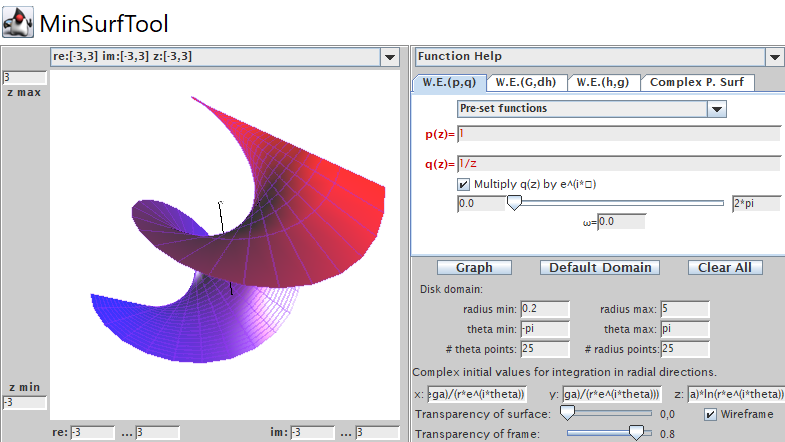
\includegraphics[scale=3]{graphs/Helicoidgraph.png}
        \caption{The helicoid using $p(z)=1$ and $q(z)=\frac{1}{z}$.}
        \label{fig:my_label}
    \end{figure}

    
  \end{block}

  \begin{alertblock}{Why Do We Care?}
    \heading{Applications of Minimal Surfaces}
    Minimal surfaces has a diverse range of applications in fields such as nanotechnology or molecular engineering and are used in physical simulation of compound polymers, black holes, soap films or protein folding.
    \heading{The Importance of Weierstrass-Enneper Parametrization}
    The Weierstrass-Enneper Parametrization guarantees that any surface created in this way by holomorphic functions is a minimal surface.
    
  \end{alertblock}

  \begin{block}{References}

    \nocite{*}
    \footnotesize{\bibliographystyle{apalike}\bibliography{poster}}

  \end{block}

\end{column}

\separatorcolumn
\end{columns}
\end{frame}

\end{document}